\section{What the existing evidence establishes}
\label{sec:evidence}

We distinguish implementations from executed results, and executed results from evidence for the proposed generalization claim. The audit pins \texttt{main} at \texttt{bdf9441a}; the four-artifact comparison is separately pinned to PR~407, commit \texttt{584713e}. These are evidence snapshots, not an assertion that an unmerged branch is part of \texttt{main}. We inspected source and receipts; we did not retrain a model or rerun a predictive benchmark for this publication. The machine-readable claim ledger records full revisions, source paths and hashes~\citep{jope,clover}.

\subsection{Working infrastructure, different claims}
The repository implements program construction, fitting, source emission, benchmark adapters and neural proposal machinery. Those capabilities make the proposed experiment plausible; they do not make its outcome known. A constrained construction can still fail compilation, execution, numerical parity or predictive evaluation. Each is a separate admission outcome, with language and operator-subset coverage recorded explicitly.

The reported CLOVER v1 outcome head attained pairwise accuracy $0.506$ (95\% lineage-bootstrap interval $[0.441,0.568]$) on fresh programs in 32 kept development contexts, compatible with chance. Later offline contextual-surrogate work reported a ranking increase of $0.046$ ($[0.040,0.052]$) across 1,136 frozen shadow contexts from 255 parents. That positive result is post-iteration shadow validation; the repository explicitly retains \texttt{flywheel\_established=false}. Neither observation licenses a universal claim that learned proposal fails or that recursive improvement succeeds. They locate an unresolved transfer problem~\citep{clover}.

The corrected public-development engine ladder reports rank 31 of 304 and Elo 1687.0, with 42/45 dataset coverage. The separately published 2259.8 rank-one row is a test-selected oracle envelope, including minima over 63,108 test-scored evaluations on 42 datasets. It is not a held-out performance result. The same-cut engine comparison reports Elo 1556.6 and rank 3 of 15, but uses ten favourably selected datasets, top-five deepening and 5/10 finalist coverage; its engine searches 32 programs across eight rounds on each cut. These are distinct experiments, none a qualified first-proposal neural evaluation. Elo values from different panels and opponent pools must not be placed on a common performance axis~\citep{jope}.

\subsection{Four frontier-labelled source artifacts}
The archived challenge fixes the target as the final column, exposes a reusable \texttt{fit}/\texttt{predict} contract, and requires safe, standalone Rust. Complete Opus-, Astra-, Sol- and Gemini-labelled source files and provenance are retained in the source appendix. The first three were present on the pinned main revision; the replacement Gemini artifact is from the separately pinned branch. Their source sizes are respectively 66,536, 27,729, 25,011 and 96,694 bytes.

Artifact identity is stronger than authoring attribution. Astra and Sol disclose prior project context, and Sol lacks exact served-model telemetry. The Gemini replacement receipt records an owner-supplied filename, with no authoring-session or exact provider/model revision evidence. These sources therefore remain historical pilots, not interchangeable pristine challenge attempts. Their use of internal validation is also relevant: frozen universal learner code may select settings while fitting. That is compatible with a no-\emph{generator}-feedback contract, but not automatically with the stronger no-algorithm-search track.

\begin{figure}[t]
  \centering
  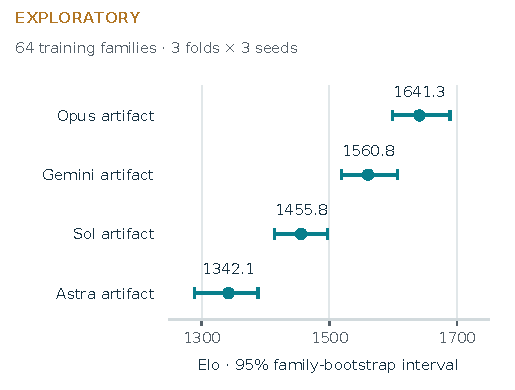
\includegraphics[width=\columnwidth]{figures/elo.pdf}
  \caption{\textbf{Exploratory artifact comparison.} Four-source Elo estimates and 95\% family-bootstrap intervals, redrawn from the pinned result receipt. There is no InnovationZero $K=1$ entrant. The panel contains 64 existing training families and prepared inner-CV contexts; preprocessing and adaptive-history caveats prevent an untouched-family claim. Short labels refer to the exact archived source IDs, not independently authenticated provider revisions.}
  \label{fig:artifact-elo}
\end{figure}

\subsection{Exploratory comparisons, with their limits}
The branch report evaluates 64 families, three folds and three seeds: 576 fitted cells per artifact. The three earlier artifacts' 1,728 fits are reused; 576 Gemini fits are added. All reported cells completed. RMSE is pooled across folds within each family and seed; Elo fits fractional, seed-averaged pairwise outcomes. The reported uncertainty resamples families 10,000 times, keeping repeated seeds together. Figure~\ref{fig:artifact-elo} reproduces the reported estimates without rerunning the fits.

The historical receipt identifies three limits that remain material despite complete coverage: these are current training families; canonical stored preprocessing was fitted before the original train/test split; and seed-41 outcomes were inspected before seeds 73 and 109 were fixed. Some inputs, prediction receipts and analysis programs remain in external custody. Thus, the figure describes these four artifacts on this exploratory panel. It does not establish performance on independent families, compare pristine models, or evaluate the proposed InnovationZero generator.

Ranking frequency and error magnitude answer different questions. Gemini's fractional match score against Sol is $65.625\%$, whereas its majority-family wins are $45/64=70.3125\%$. The oriented geometric-mean error ratio is $\mathrm{RMSE}_{\mathrm{Sol}}/\mathrm{RMSE}_{\mathrm{Gemini}}=0.8468$ (95\% interval $[0.6234,1.0554]$): Gemini's point estimate is about $18.1\%$ higher, not $15\%$. The interval crosses parity, and none of the three reported Gemini comparisons is significant after its stated Holm adjustment. The source appendix preserves original receipts unchanged; this interpretation corrects their compressed prose.

Finally, Gemini's 1,985.8 seconds of aggregate fitting came from a different host than the historical fits. It cannot support a controlled speed ratio. Historical effort report C is linked to Opus by the repository record; report D remains unattributed and is not assigned to Gemini by resemblance of names. These limits motivate the prospective, failure-inclusive protocol rather than diminishing the value of preserving the observations.
